\uuid{roOt}
\exo7id{5121}
\titre{exo7 5121}
\auteur{rouget}
\organisation{exo7}
\datecreate{2010-06-30}
\isIndication{false}
\isCorrection{true}
\chapitre{Nombres complexes}
\sousChapitre{Racine carrée, équation du second degré}
\module{Algèbre}
\niveau{L1}
\difficulte{}

\contenu{
\texte{

}
\begin{enumerate}
    \item \question{On pose $z=e^{2i\pi/5}$ puis $a=z+z^4$ et $b=z^2+z^3$. Déterminer une équation du second degré dont les
solutions sont $a$ et $b$ et en déduire les valeurs exactes de $\cos\left(\frac{2\pi}{5}\right)$, $\sin\left(\frac{2\pi}{5}\right)$,
$\cos\left(\frac{4\pi}{5}\right)$, $\sin\left(\frac{4\pi}{5}\right)$, $\cos\left(\frac{\pi}{5}\right)$ et $\sin\left(\frac{\pi}{5}\right)$.}
\reponse{On a $a=2\cos\left(\frac{2\pi}{5}\right)$ et $b=2\cos\left(\frac{4\pi}{5}\right)$. $1$, $z$, $z^2$, $z^3$ et $z^4$ sont les cinq
racines cinquièmes de $1$ dans $\Cc$. Par suite, $1+z+z^2+z^3+z^4=0$. Mais alors

$$a+b=z+z^2+z^3+z^4=-1$$
et

$$ab=(z+z^4)(z^2+z^3)=z^3+z^4+z^6+z^7=z+z^2+z^3+z^4=-1\;(\mbox{car}\;z^5=1).$$
$a$ et $b$ sont donc les solutions de l'équation $X^2+X-1=0$ dont les racines sont $\frac{-1+\sqrt{5}}{2}$ et
$\frac{-1-\sqrt{5}}{2}$. Enfin, puisque $\frac{2\pi}{5}\in\left]0,\frac{\pi}{2}\right[$, on a $a>0$. Par
suite, $\cos\left(\frac{2\pi}{5}\right)=\frac{-1+\sqrt{5}}{4}$ et $\cos\left(\frac{4\pi}{5}\right)=\frac{-1-\sqrt{5}}{4}$. D'autre part,
$\sin\left(\frac{2\pi}{5}\right)>0$ et donc,

$$\sin\left(\frac{2\pi}{5}\right)=+\sqrt{1-\cos^2(\frac{2\pi}{5})}=\sqrt{1-\left(\frac{-1+\sqrt{5}}{4}\right)^2}=\frac{1}{4}
\sqrt{10+2\sqrt{5}}.$$

\begin{center}
\shadowbox{
$\cos\left(\frac{2\pi}{5}\right)=\frac{\sqrt{5}-1}{4}$ et $\sin\left(\frac{2\pi}{5}\right)=\frac{1}{4}
\sqrt{10+2\sqrt{5}}$.
}
\end{center}
De même, en remplaçant $\sqrt{5}$ par $-\sqrt{5}$, $\cos\left(\frac{4\pi}{5}\right)=\frac{-1-\sqrt{5}}{4}$ et
$\sin\left(\frac{4\pi}{5}\right)=\frac{1}{4}\sqrt{10-2\sqrt{5}}$. Enfin,
$\cos\left(\frac{\pi}{5}\right)=-\cos\left(\pi-\frac{\pi}{5}\right)=-\cos\left(\frac{4\pi}{5}\right)=\frac{1+\sqrt{5}}{4}$
et $\sin\left(\frac{\pi}{5}\right)=\sin\left(\pi-\frac{\pi}{5}\right)=\sin\left(\frac{4\pi}{5}\right)=\frac{1}{4}\sqrt{10-2\sqrt{5}}$.\rule[-5mm]{0mm}{0mm}}
    \item \question{Le cercle de centre $\Omega$ d'affixe $-\frac{1}{2}$ passant par le point $M$ d'affixe $i$ recoupe 
$(Ox)$ en deux points $I$ et $J$. Montrer que
$\overline{OI}+\overline{OJ}=\overline{OI}.\overline{OJ}=-1$ et en déduire une construction à la règle et au
compas, du pentagone régulier
inscrit dans le cercle de centre $O$ et de rayon $1$ dont un des sommets est le point d'affixe $1$.\rule[-1mm]{0mm}{0mm}}
\reponse{Le rayon du grand cercle vaut, d'après le théorème de \textsc{Pythagore}~:

$$R=\sqrt{\Omega O^2+OM^2}=\frac{\sqrt{5}}{2}.$$
Donc $x_I=x_\Omega+R=\frac{-1+\sqrt{5}}{2}$ et $x_J=x_\Omega-R=\frac{-1-\sqrt{5}}{2}$. Par suite,
$x_I=2\cos\left(\frac{2\pi}{5}\right)$ et $x_J=2\cos\left(\frac{4\pi}{5}\right)$. Ceci montre que les médiatrices des segments $[O,I]$ et
$[O,J]$ coupent le cercle de centre $O$ et de rayon $1$ en quatre des cinq sommets du pentagone.

$$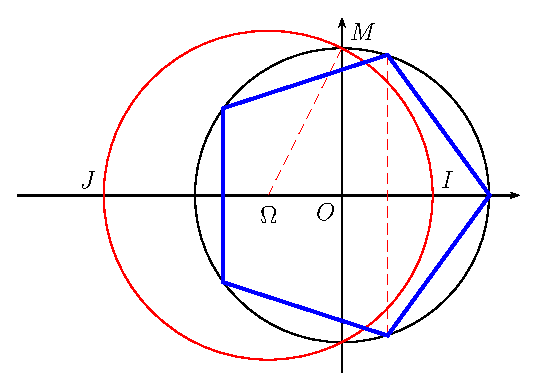
\includegraphics{../images/img005121-1}$$}
    \item \question{La diagonale $[AC]$ d'un pentagone régulier $(ABCDE)$ est recoupée par deux autres diagonales en deux points
$F$ et $G$. Calculer les rapports $\frac{AF}{AC}$ et $\frac{FG}{AF}$.}
\reponse{Posons $x=\frac{AF}{AC}$. D'après le théorème de \textsc{Thales} (je vous laisse
vérifier les parallélismes),
$$x=\frac{AF}{AC}=\frac{HK}{HC}=\frac{FG}{FC}=\frac{AC-2AF}{AC-AF}=\frac{1-2x}{1-x}.$$
Donc $x^2-3x+1 = 0$ et puisque $x<1$, $x=\frac{3-\sqrt{5}}{2}$. Puis

$\frac{AG}{AC}=\frac{AC-AF}{AC}=1-x=\frac{-1+\sqrt{5}}{2}$ et
$\frac{FG}{AF}=\frac{AC-2AF}{AF}=\frac{1}{x}-2=\frac{2}{3-\sqrt{5}}-2=\frac{3+\sqrt{5}}{2}-2=\frac{-1+\sqrt{5}}{2}
$.

$$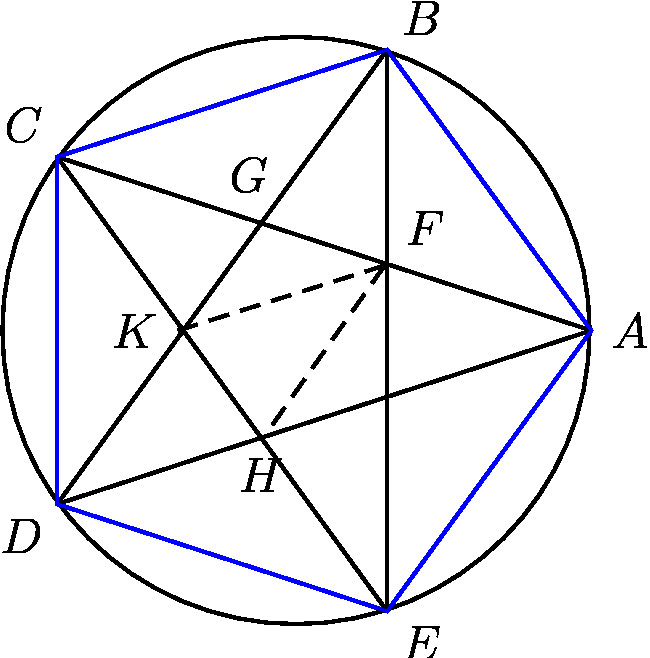
\includegraphics{../images/img005121-2}$$

Définition du \emph{nombre d'or}.

$$
\includegraphics{../images/img005121-3}$$

On veut que $C$ partage le segment $[A,B]$ de telle sorte que $\frac{BC}{AC}=\frac{AC}{AB}$
(\og~$\frac{\mbox{petit}}{\mbox{moyen}}=\frac{\mbox{moyen}}{\mbox{grand}}$~\fg) c'est-à-dire, en posant $a=AB$ et
$x=AC$, $\frac{x}{a}=\frac{a-x}{x}$ ou encore $\left(\frac{x}{a}\right)^2+\frac{x}{a}-1=0$ et donc, puisque $\frac{x}{a}>0$,
$\frac{x}{a}=\frac{-1+\sqrt{5}}{2}$. 

\begin{center}
\shadowbox{
Le nombre d'or (ou proportion dorée) est le 
nombre $\frac{-1+\sqrt{5}}{2}=0,618...$
}
\end{center}
On peut aussi prendre pour le nombre d'or le
rapport $\frac{a}{x}=\frac{1+\sqrt{5}}{2}=1,618...$}
\end{enumerate}
}
